\newpage
\section{Auswertung}
Die Schallgeschwindigkeit in Acryl kann mit Formel %(\ref{eqn:c})
bestimmt werden.
Wird der doppelte Abstand $d$, die Strecke die der Ultraschall tatsächlich zurücklegt,
gegen die Zeit $t$ geplottet die er dafür benögtigt, ist die Steigung der Ausgleichsgeraden
die Schallgeschwindigkeit.

\noindent
Mittels Python kann die Ausgleichsgerade mit der aus numpy \cite{numpy} importierten Funktion polyfit bestimmt werden.
Diese ist in Abbildung (\ref{fig:schall}) dargestellt.

\begin{figure}
    \centering
    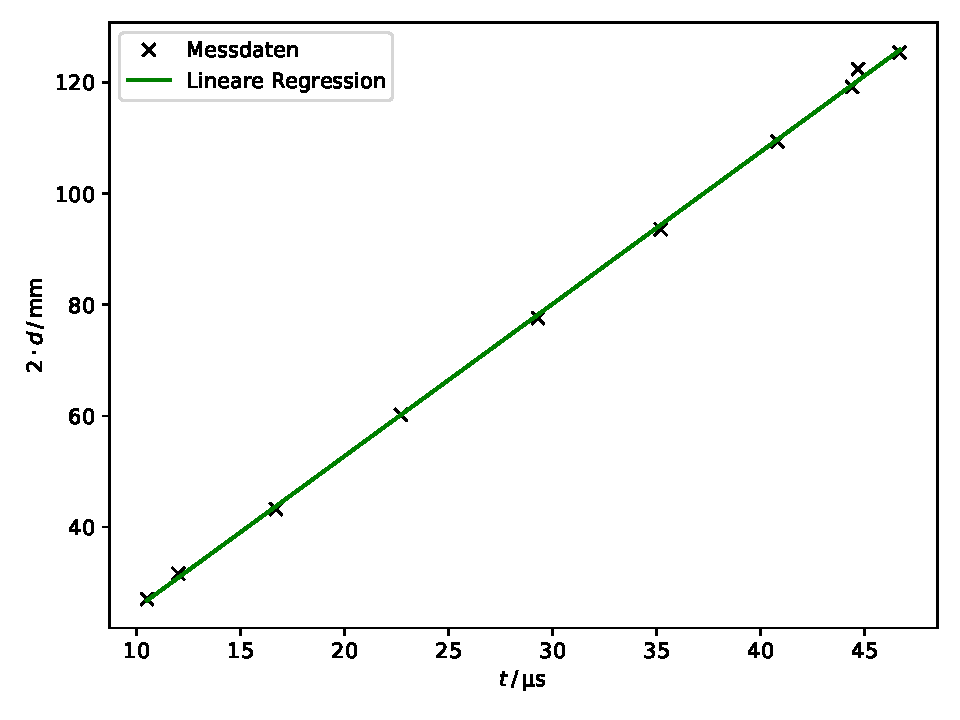
\includegraphics[width=9cm]{schall.pdf}
    \caption{Ausgleichsgerade zur Bestimmung der Schallgeschwindigkeit (Quelle:\cite{US1}).}
    \label{fig:schall}
  \end{figure}
  
\noindent
Die Ausgleichsgerade hat dabei die Funktionsvorschrift:

\begin{align*}
2 \cdot d(t) &= 2.7372 \, \si[per-mode=fraction]{\milli\meter\per\micro\second} \cdot t \\
\implies c_{Acryl} &= 2732.2 \, \si[per-mode=fraction]{\meter\per\second} \\
\end{align*}

\noindent
Die Dämpungskonstante aus Formel () lässt sich bestimmen, indem die Messwerte aus Tabelle () an eine Exponentialfunktion gefittet werden.
Mit Python kann eine e-Funktion mit passenden Parametern mit der aus scipy \cite{scipy} importierten Funktion curvefit bestimmt werden.

\begin{figure}
    \centering
    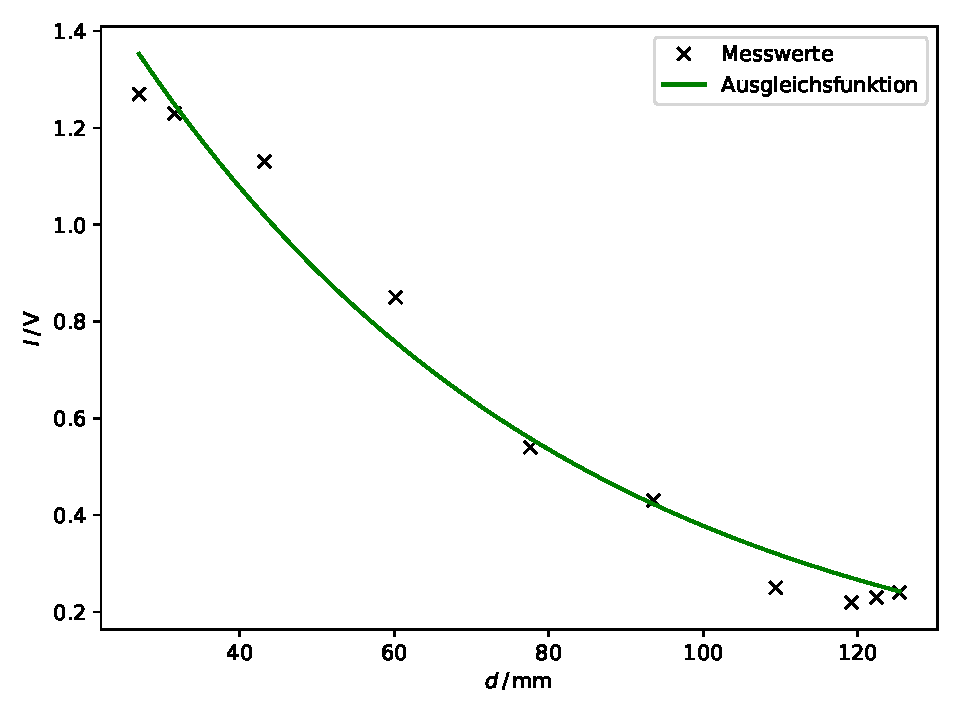
\includegraphics[width=9cm]{daempf.pdf}
    \caption{Ausgleichsfunktion zur Bestimmung der Dämpfungskonstante (Quelle:\cite{US1}).}
    \label{fig:daempf}
  \end{figure}

\noindent
Die in Abbildung (\ref{fig:daempf}) dargestellt Ausgleichsfunktion hat die Funktionsvorschrift:

